%!TEX program = xelatex
%!TEX root = ../thesis.tex
\chapter{Introduction}

Environmental issues are always a big part of scientific research for our human beings, among which the air pollution problem is a big head. Due to the increasing of industries and usage of fossil energy, and emission of industrial wastewater, and so on, many kinds of air pollutants such as carbon dioxide, sulfur oxides, nitrogen oxides, carbon monoxide, volatile organic compounds, and particulate matter have been main sources for the air pollution \cite{kampa_human_2008}.

As World Health Organization (WHO) states \cite{world2016ambient}, air pollution is the world's largest environmental health risk. And air pollution is a significant risk factor for many pollution-related diseases, including but not limited to respiratory infections, heart disease, COPD, stroke, and lung cancer. It has the largest impact on premature deaths annually \cite{lelieveld2015contribution}. Hence, as people's awareness of health-related problems increases, more smart and wearable devices have been developed. An example of smart wearable devices is the smart band. It can retrieve air quality status from the Internet and report it to the user. Another example of smart home devices is the smart indoor air purifier that can automatically purify the air when detecting high AQI levels during the resident's absence.

% 空气污染相关的work,因为是Intro,所以可以说得简短一点
The air pollution problem leads to many research work topics such as AIoT and sensing networks. Kumar et al. \cite{kumar2017air}, Oh et al. \cite{oh2015indoor}, Zheng et al. \cite{zheng2016design}, and many others designed different kinds of AIoT systems to monitor air quality, feature by variant function and application scenario. Ray et al. \cite{ray2016internet} built a smart airborne PM2.5 density monitoring system based on the cloud platform. However, to drive the purifier to turn on\/off or onto different power levels, the first problem is to let the purifier know the current air pollution level and predict the trend. The control feedback can be illustrated as Figure \ref{fig:greeneyes_aiot} shows.

This thesis presents GreenEyes, an air pollution evaluation system based on WaveNet, a versatile and end-to-end deep learning network. Our system can monitor and collect real-time PM2.5 and PM10 data and illustrate them to multiple end-users. Moreover, when added with other smart devices such as indoor air purifiers or a smart wearable helmet, it can form an air monitoring and purifying smart IoT system.

% TODO 属于讨论,不该放在这里 这段要过一下Grammarly
% However, firstly, these air monitoring solutions are not oriented for mobility demands; they put the sensors at a fixed monitoring spot. Secondly, most of them use just one air quality sensor at the same place; even for the approach of networked solutions, it uses only one sensor at each place either.

\begin{figure}[!htbp]
    \begin{center}
    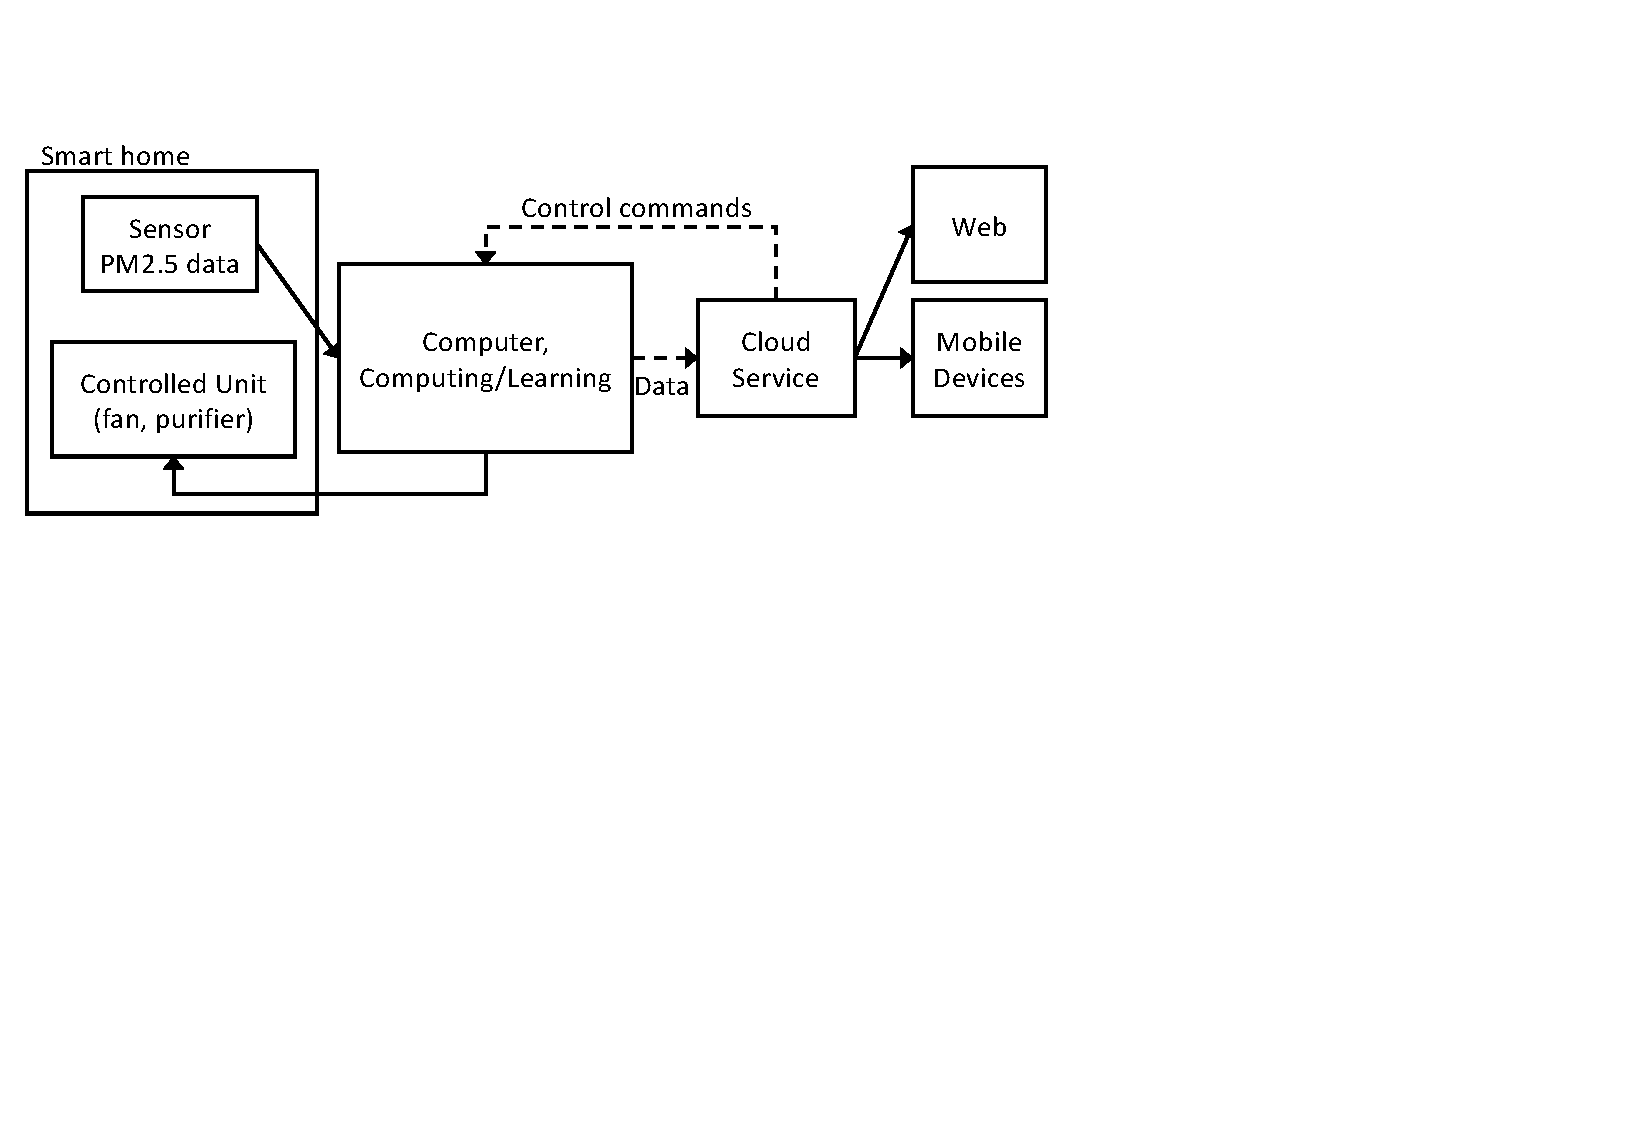
\includegraphics[width=\linewidth]{slides/pdf/greeneyes_aiot.pdf}
    \end{center}
    \caption{GreenEyes: AIoT deployment.}
    \label{fig:greeneyes_aiot}
\end{figure}

In this work, we investigated preprocessing noisy PM2.5\/10 sequence data and creating appropriate supervising data. We designed and implemented the GreenEyes model, applied it to AQI level fitting and predicting. We not only evaluated it on every single channel of PM2.5 data but also trained our model with all channels' data together. Other people's work either uses different kinds of data \cite{han2020joint}, or use sensors of the same model but place them at different places \cite{ray2016internet}. The former methodology is Multi-sensor Fusion \cite{wang2019multi}, it is widely used in intelligent and autonomous systems \cite{luo1989multisensor} \cite{hall1997introduction} \cite{wang2012towards} \cite{cai2020probabilistic}. However, our experiment approach tries to prove that multi-sensors of the same model placed at the same place will make the fitting model more robust.

\textbf{Organization:} Chapter 1 has already given the background introduction. The remainder of this thesis is organized as follows. In Chapter 2, we will present some preliminaries. Chapter 3 will introduce related works. In Chapter 4, we will illustrate our GreenEyes model. Contents of Chapters 5 and 6 are experiment procedures and results. In Chapter 7, we will discuss this thesis about its application outlooks and future works. Finally, Chapter 8 concludes this thesis.
